\section{Elettronica, Programmazione e Sviluppo di Prototipi}
%
Oltre alle attività legate alla pura modellazione e fabbricazione, una parte essenziale del tirocinio si è concentrata sull'integrazione hardware-software. Questo mi ha permesso di approfondire in modo pratico e sul campo l'elettrotecnica e la programmazione, unendo la parte hardware con quella software nei progetti.

%
\subsection{Elettrotecnica e prototipazione}
Ho affinato le mie competenze nella realizzazione di circuiti elettronici, partendo dalla prototipazione su breadboard fino ad arrivare alla saldatura a stagno definitiva dei componenti. Questa fase operativa è stata costantemente accompagnata da un'attività di diagnostica e troubleshooting: ho imparato a eseguire test su alimentatori, circuiti e monitor, verificandone tensioni, continuità e segnali per individuare eventuali malfunzionamenti hardware prima dell'assemblaggio finale.
%
\subsection{Programmazione di microcontrollori}
Sul fronte software, ho lavorato estensivamente con schede Arduino (utilizzando il suo linguaggio nativo) e single-board computer come il Raspberry Pi (sviluppando principalmente script in Python).
L'ambiente stimolante del Fablab mi ha inoltre permesso di dedicare parte del tempo a progetti di ricerca e sviluppo personale, sfruttando i linguaggi di programmazione per creare soluzioni ``custom''. Il progetto più significativo in questo senso è stato l'ideazione di un ipotetico Heads-Up Display (HUD) per la mia autovettura (Peugeot 208). Utilizzando Python e Arduino, ho studiato come gestire il flusso di dati e l'interfaccia visiva per proiettare le informazioni utili sul parabrezza, dimostrando come le tecnologie maker possano essere applicate per creare soluzioni innovative anche in ambito automotive.

Ho esteso inoltre le mie competenze all'automazione dei flussi di lavoro e allo sviluppo di tooling in ambiente macOS. Per ottimizzare la stesura e la gestione dei miei appunti accademici in \LaTeX, ho progettato un'infrastruttura di lavoro personalizzata.
Nello specifico, ho strutturato un ambiente organizzato in directory e lo ho caricato sulla mia pagina di GitHub, ospitando la repository per garantire il tracciamento delle modifiche e l'accessibilità dei materiali dei miei corsi.

Per rendere questo ecosistema rapido ed efficiente, ho ideato e programmato in prima persona degli script da riga di comando (CLI):

\begin{itemize}
    \item \verb|makecourse|: uno script progettato per automatizzare l'inizializzazione di un nuovo corso, generando istantaneamente l'alberatura delle cartelle e i file template di base.
    \item \verb|makelecture|: uno strumento più avanzato dedicato alla gestione dinamica dei file \LaTeX  \, delle singole lezioni. Lo script è stato programmato per accettare argomenti posizionali (come il titolo della lezione per la sua creazione automatica) e diverse opzioni flag, tra cui la rimozione sicura di lezioni esistenti (-r o --remove), l'elencazione dei file generati (-l o --list) e il controllo di versione (-v).
\end{itemize}

Lo sviluppo di questi strumenti mi ha permesso di approfondire in modo significativo lo scripting da terminale, la creazione di interfacce a riga di comando (CLI) e l'importanza dell'ottimizzazione e del controllo di versione nella gestione dei progetti software e documentali.

\begin{figure}
    \centering
    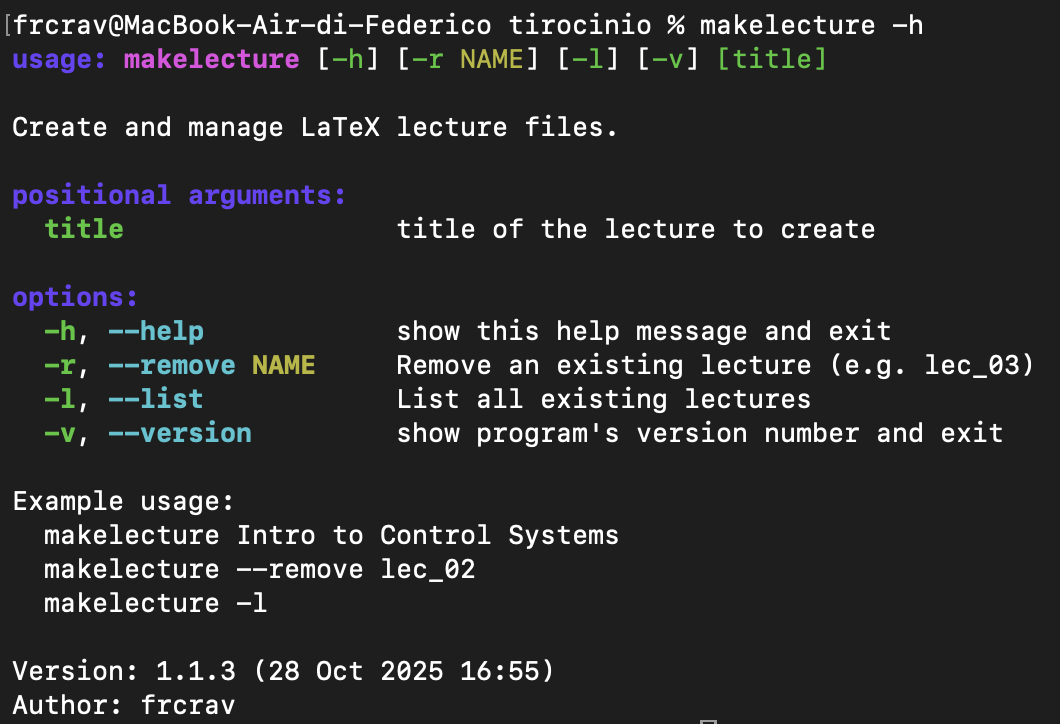
\includegraphics[width=0.6\linewidth]{assets/Screenshot 2026-05-13 at 10.41.34.png}
    \caption{CLI per \LaTeX}\label{fig:}
\end{figure}

\progetto{Cabinato Arcade}{Autonomo, Mar 2026}
Ho partecipato attivamente alla riparazione e alla costruzione di un sistema arcade. Mi sono occupato del cablaggio interno dei pulsanti e dei joystick, dell'adattamento e dell'integrazione del monitor, e dell'interfacciamento di tutta l'elettronica di controllo con il ``cervello'' del sistema.

\progetto{Drone FPV da 150mm}{Gruppo Cipro, Nov 2025}
Durante il workshop ho introdotto la prototipazione di un drone classe 150mm. La realizzazione di questo dispositivo ha richiesto un'elevata precisione nella saldatura della componentistica di volo (motori brushless, ESC, flight controller e riceventi radio) e un'attenta analisi della distribuzione energetica all'interno di un sistema compatto e ad alto assorbimento. Sebbene la complessità tecnica e le tempistiche del progetto si siano rivelate superiori agli obiettivi didattici previsti per gli studenti, ho deciso di proseguirne lo sviluppo in autonomia. Questa scelta mi ha permesso di trasformare l'attività in un prezioso progetto di ricerca personale, approfondendo in chiave propedeutica le complesse dinamiche costruttive ed elettroniche dei velivoli a pilotaggio remoto. \\ Vedi figura \ref{fig:drone}.
\begin{figure}
    \centering
    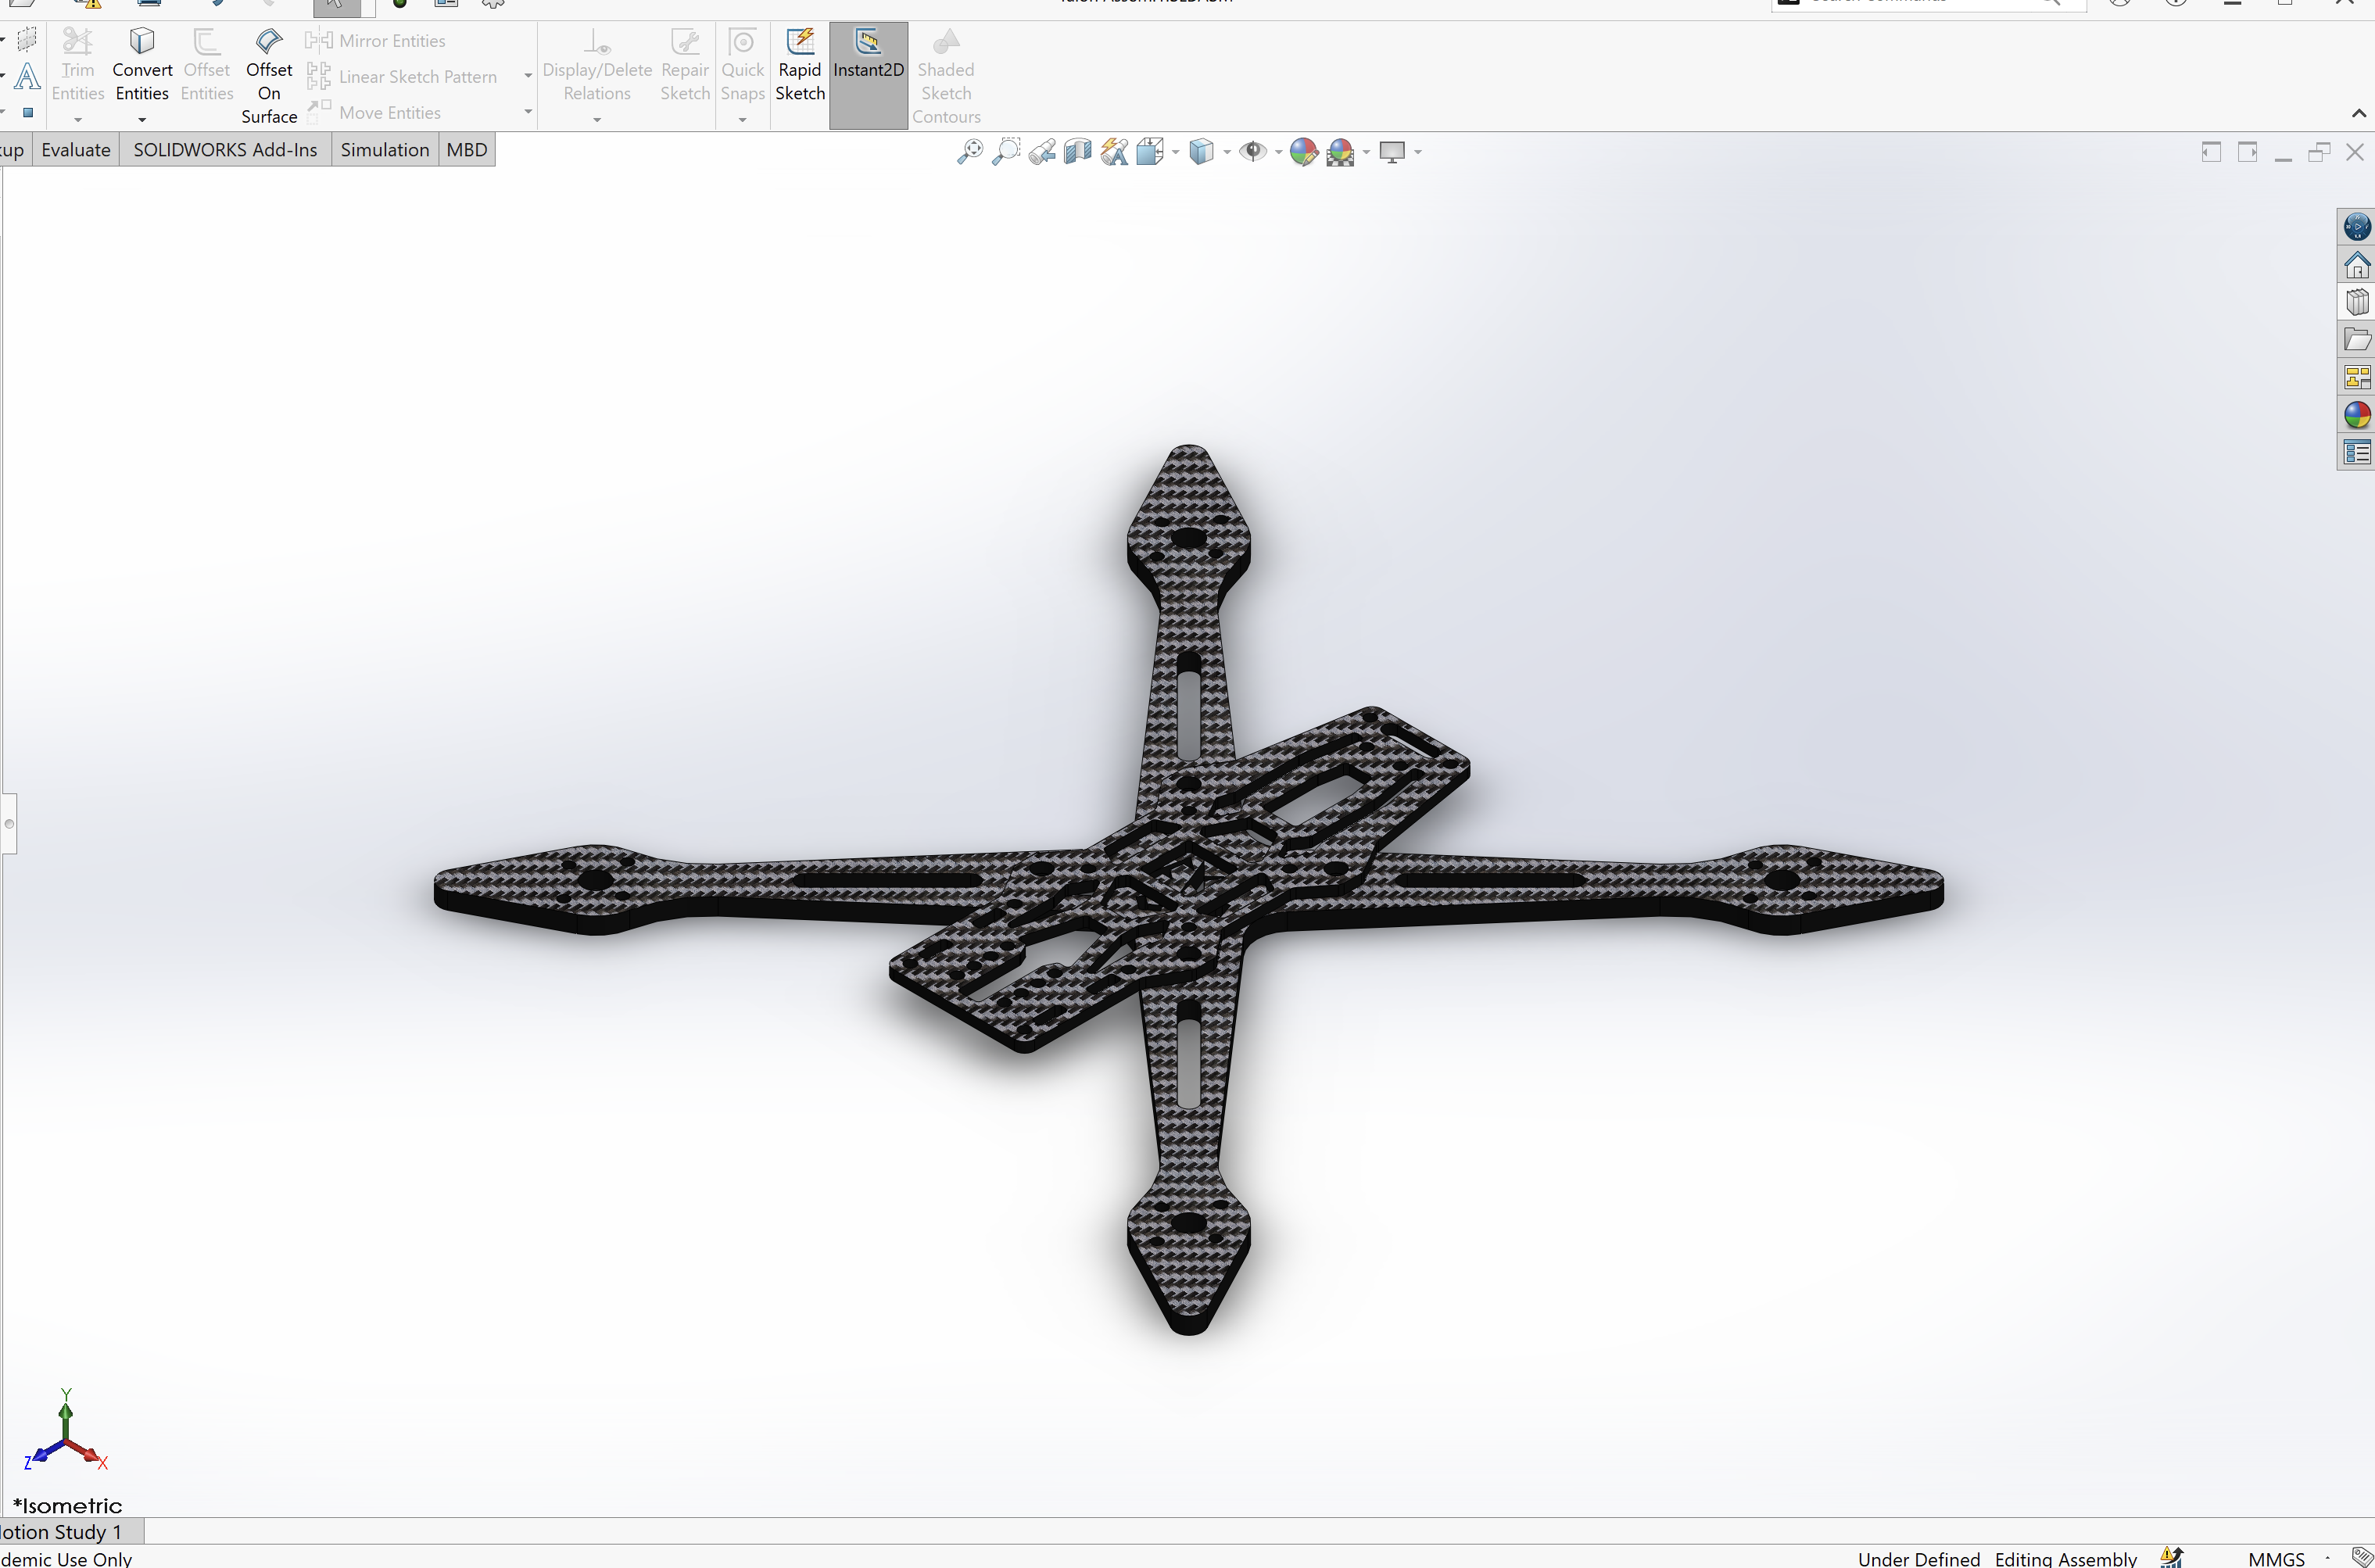
\includegraphics[width=1\linewidth]{assets/image.png}
    \caption{Drone FPV, gruppo Cipro}\label{fig:drone}
\end{figure}


\progetto{Heads-Up Display}{Autonomo, Nov 2025}
Utilizzando Python e Arduino, ho studiato come gestire un ipotetico flusso di dati e un'interfaccia visiva per proiettare le informazioni utili sul parabrezza della mia autovettura, dimostrando come le tecnologie maker possano essere applicate per creare soluzioni innovative anche in ambito automotive.
Il progetto è nato da una forte spinta autodidatta, motivata dal desiderio di realizzare un sistema personalizzato in grado di proiettare direttamente sul parabrezza i dati di telemetria dell'autovettura e le indicazioni di navigazione.

Considerando che l'HUD è solitamente un optional riservato a vetture di fascia alta, ho voluto sfruttare l'approccio maker per progettare una soluzione accessibile e integrare questa tecnologia sulla mia utilitaria.